\documentclass[a4paper,12pt]{article}
\usepackage[utf8]{inputenc}
\usepackage[brazil]{babel}
\usepackage[margin = 2cm]{geometry}
\usepackage{amsmath}
\usepackage{graphicx}
\usepackage{subfigure}
\usepackage{listings}
\usepackage{amssymb}
\usepackage{array}
\usepackage{indentfirst}
\usepackage{textcomp}
\usepackage{pdfpages}
\usepackage[backend=biber, sorting=none]{biblatex}
\usepackage{helvet}
\usepackage{palatino}
%\usepackage[table,xcdraw]{xcolor}

\usepackage{caption}
% \usepackage{floatrow}
\usepackage[capposition=top]{floatrow}

% aspas
\usepackage{csquotes}
\MakeOuterQuote{"}

\renewcommand{\familydefault}{\sfdefault}

\bibliography{bibliografia.bib}

%aspell --lang=pt_BR --master=pt_BR --mode=tex -c relatorio-parcial.tex

\begin{document}

  \begin{titlepage}
    \begin{center}
    \begin{minipage}[t]{0.74\textwidth}
    \vspace{0pt}
    \begin{center}
     UNIVERSIDADE FEDERAL DO PARANÁ \\
     SETOR DE TECNOLOGIA \\
     DEPARTAMENTO DE ENGENHARIA ELÉTRICA
    \end{center}
    \end{minipage}\\[1.5cm]

    {{WENDEURICK EMERICK SILVERIO\\GRR20134722}}\\[3cm]

    {\Large{Proposta do Projeto de Graduação}}\\[1cm]
    {\Large \textbf{Desenvolvimento de Mesa de Luz Interativa para Experimento de Ciências para Crianças}}\\[2.5cm]


      \hspace{.45\textwidth} %posiciona a minipage
       \begin{minipage}{.5\textwidth}
       Plano do Trabalho de Conclusão de Curso, apresentado como requisito parcial para a obtenção do grau de Engenheiro Eletricista, no programa de graduação em Engenharia Elétrica (ênfase em Eletrônica e Telecomunicações) da Universidade Federal do Paraná.\\
       \\
       Orientador: Prof. Dr. James Alexandre Baraniuk
       
      \end{minipage}
      \\[6.5cm]

      {\textbf{CURITIBA}}\\
      {2018}


    \end{center}
  \end{titlepage}

  \tableofcontents

  \clearpage
  \section{Contextualização e Resumo}
  
  A luz exerce um papel essencial no nosso cotidiano e está presente das mais diversas formas: iluminação, medicina, pesquisas científicas, geração de energia, telecomunicações, educação, arte, cultura e etc. A Assembleia Geral das Nações Unidas proclamou o ano de 2015 como o Ano Internacional da Luz e das Tecnologias Baseadas na Luz \cite{resolucao-onu}, a fim de reconhecer tal importância para a vida dos cidadãos e para o desenvolvimento futuro da sociedade mundial. No ano da celebração, a UNESCO promoveu uma série de eventos por vários países \cite{eventos-unesco}, com o intuito de destacar que o aumento da consciência mundial e o fortalecimento do ensino da ciência e das tecnologias da luz são essenciais para abordar os desafios futuros e atuais, tais como o desenvolvimento sustentável, a energia e as comunicações, assim como para melhorar a qualidade de vida dos países menos desenvolvidos e dos em desenvolvimento.
  
  Baseada em tal iniciativa, a exposição "Luz, Ciência e Emoção", idealizada pela arquiteta Dra. Maristela Mitsuko Ono e pelo engenheiro Dr. James Alexandre Baraniuk, traz experimentos envolvendo os conceitos de luz trabalhados nos ensinos pré-escolar e fundamental, cada um com seu grau de impressão aos sentidos. A exposição proporciona uma experiência tangível-visual impactante aos observadores, causando deslumbramento e entusiasmo através da arte e interação.
  
  O trabalho aqui proposto trata-se do desenvolvimento do \emph{hardware} e \emph{firmware} embarcado de um dos mais de 20 experimentos dessa exposição. A \textbf{Mesa de Bolinhas}, que se enquadra na área artística da mostra, é uma matriz de \emph{LEDs} interativa, elaborada pela arquiteta Dra. Maristela Mitsuko Ono, composta por mais de 100 bolinhas de ping-pong, cada uma correspondente a um par LED-sensor reflexivo. Ela permite que o visitante "pinte com luz" ao passar a mão sobre a mesa. Sua vista superior do projeto é apresentada na Figura \ref{fig:mesa-sup}.
  	
  \begin{figure}[H]
    \caption{Vista superior da mesa}
    \label{fig:mesa-sup}
    \centering
    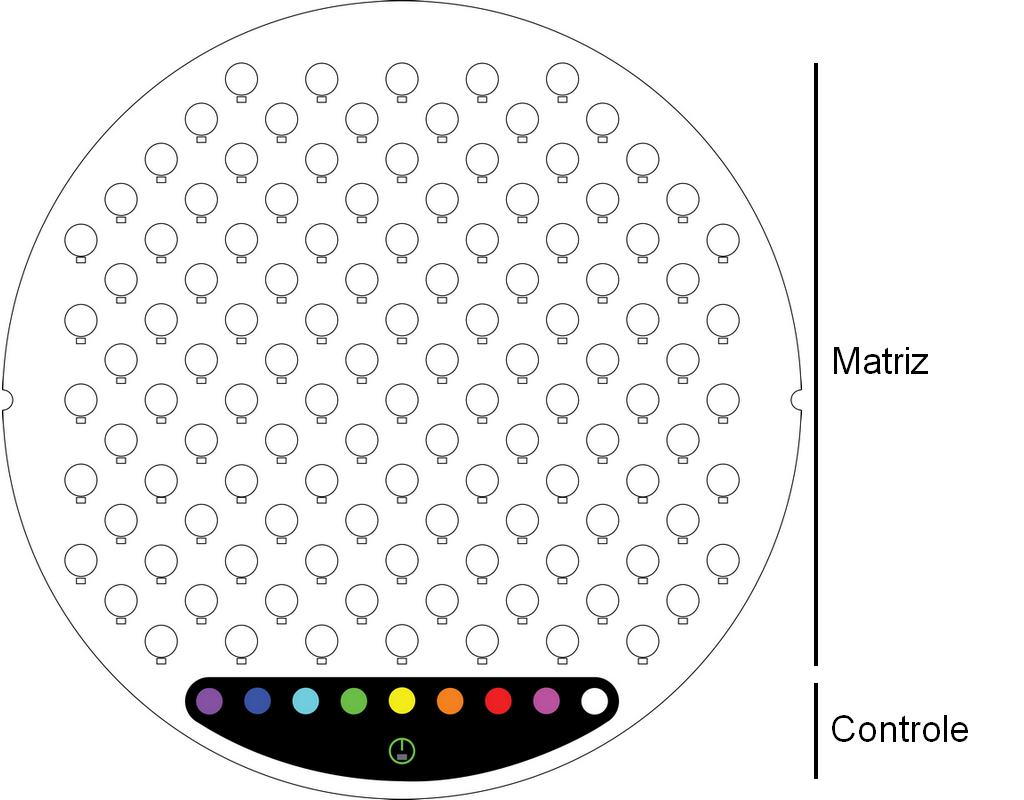
\includegraphics[width=0.7\linewidth]{img/mesa-cad.png}
    \floatfoot{Fonte: (MITSUKO, 2016)}
  \end{figure}	
	
	
  \clearpage
  
  \section{Proposta de Trabalho}
  
  \subsection{Título}
  
  \emph{Desenvolvimento de Mesa de Luz Interativa para Experimento de Ciências para Crianças}.
  
  \subsection{Objetivos}
  \subsubsection{Objetivo Geral}
  
  Desenvolver o \emph{hardware} e o \emph{firmware} embarcado da "Mesa de Bolinhas", apresentando o protótipo funcional do projeto. Serão 128 LEDs programáveis, controlados por seus respectivos sensores de presença.
  
  \subsubsection{Objetivos Específicos}
  \begin{itemize}
      \item Desenvolvimento de uma matriz mapeável, onde cada \emph{LED} possa ser controlado individualmente;
      \item Desenvolvimento de uma matriz de entrada, onde cada sensor reflexivo possa ser lido individualmente;
      \item \emph{Software} microcontrolado que gerencie a interface humano-máquina;
      \item Leiaute e montagem das Placas de Circuito Impresso (PCI);
      \item Integração da eletrônica com a mecânica do projeto.
  \end{itemize}
  
  \subsection{Público Alvo}
  A serventia do projeto é destinada ao mesmo público alvo da exposição: crianças e adolescentes dos ensinos fundamental e médio. Além disso, o projeto pode ser de interesse de designers e artistas, uma vez que abrange áreas de tecnologia, interação e arte generativa.
  
  \subsection{Diferencial do Projeto}
  Além de ser uma matriz interativa autônoma, a Mesa de Bolinhas terá uma interface que possibilitará o controle através de outros dispositivos (computador, por exemplo). Isso possibilitará a integração com programas de \emph{led-mapping} e geradores de visuais.
  
  Tratando-se de uma proposta inovadora, pretende-se solicitar a patente do projeto.
  
  \subsection{Metodologia de desenvolvimento do estudo}
  A metodologia se dará por meio de protótipos, servindo de prova de conceito. Logo após, passa-se à implementação e execução do projeto.
  
\subsection{Recursos necessários}

Os materiais (mesa, tampa acrílica e demais partes mecânicas) já foram adquiridos pelo curso de Engenharia Elétrica, através do prof. James Baraniuk, e estão no Laboratório de Eficiência Energética. O projeto encontra-se sem o dispositivo eletrônico, cuja proposta deste trabalho é de desenvolvê-lo e integrá-lo à parte mecânica. Para isso, serão necessários:

\begin{itemize}
    \item \emph{Software CAD} para o leiaute das placas;
    \item Material para fabricação dos protótipos (PCIs, LEDs programáveis (WS2812) e demais componentes eletrônicos);
    \item Plataforma de desenvolvimento (microcontrolador da família ESP8266);
\end{itemize}

\subsection{Resultados fundamentais a serem atingidos}
Protótipo funcional da Mesa de Bolinhas, montagem das PCIs e integração com a mecânica do projeto.

\subsection{Contribuição esperada para a ênfase}
A nível geral, o projeto contribui no quesito integração com a área artística e de design. A nível técnico, o projeto trará recursos/implementações de mapeamento de \emph{pixels}, sistema de \emph{debouncing} para vários sensores, implementação de \emph{software} desenvolvido em topologia de Máquina de Estados Finita e etc.

\subsection{Cronograma a ser seguido indicando os marcos para avaliação, seguindo o cronograma divulgado pela Comissão Permanente do TCC}

\begin{table}[H]
\begin{tabular}{|l|c|c|c|c|}
\hline
\textbf{Atividade/Mês}        & \textbf{Agosto} & \textbf{Setembo} & \textbf{Outubro} & \textbf{Novembro} \\ \hline
\textbf{Atividade 1}          & X               & X                &                  &                   \\ \hline
\textbf{1ª Avaliação}         &                 & X                &                  &                   \\ \hline
\textbf{Atividade 2}          &                 & X                & X                &                   \\ \hline
\textbf{Banca}                &                 &                  & X                &                   \\ \hline
\textbf{Atividade 3}          &                 &                  & X                & X                 \\ \hline
\textbf{Entrega do Relatório} &                 &                  &                  & X                 \\ \hline
\textbf{Apresentação Final}   &                 &                  &                  & X                 \\ \hline
\end{tabular}
\end{table}

\begin{itemize}
    \item Atividade 1: desenvolvimento da seção "Matriz" 
    \item Atividade 2: desenvolvimento da seção "Controle"
    \item Atividade 3: finalização e integração com a mecânica
\end{itemize}

\subsection{Importância do Projeto para a formação dos autores}
Para o aluno, o conhecimento aqui adquirido é de fundamental importância para sua formação e interdisciplinaridade, uma vez que abrange resolução de problemas no campo da engenharia eletrônica / sistemas embarcados e o intercâmbio com outras áreas.


Para os idealizadores, o projeto passará a ser parte da exposição "Luz, Ciência e Emoção", proporcionando uma experiência tangível-visual impactante aos observadores, causando deslumbramento e entusiasmo através da arte e interação, não só das crianças e adolescente, mas também de pessoas que se interessem pela integração entre tecnologia, arte e design.

\subsection{Bibliografia a ser utilizada}

\begin{itemize}
    \item GAMMA, Erich et al. \textbf{Design Patterns}: Elements of Reusable Object-Oriented Software. 10. ed. Mountain View: Addison-Wesley Professional, 1994. 416 p.
    
    \item WAGNER, Ferdinand et al. \textbf{Modeling Software with Finite State Machines}. 1. ed. Boston: Auerbach Publications, 2006. 390 p.
\end{itemize}

 \clearpage
  
  
  \clearpage
  \section{Referências}
  \printbibliography

\end{document}
